\section{Appendix 1 - Frequency distribution of observed variables} \label{appendixa}

\begin{figure}[H]
\centering
	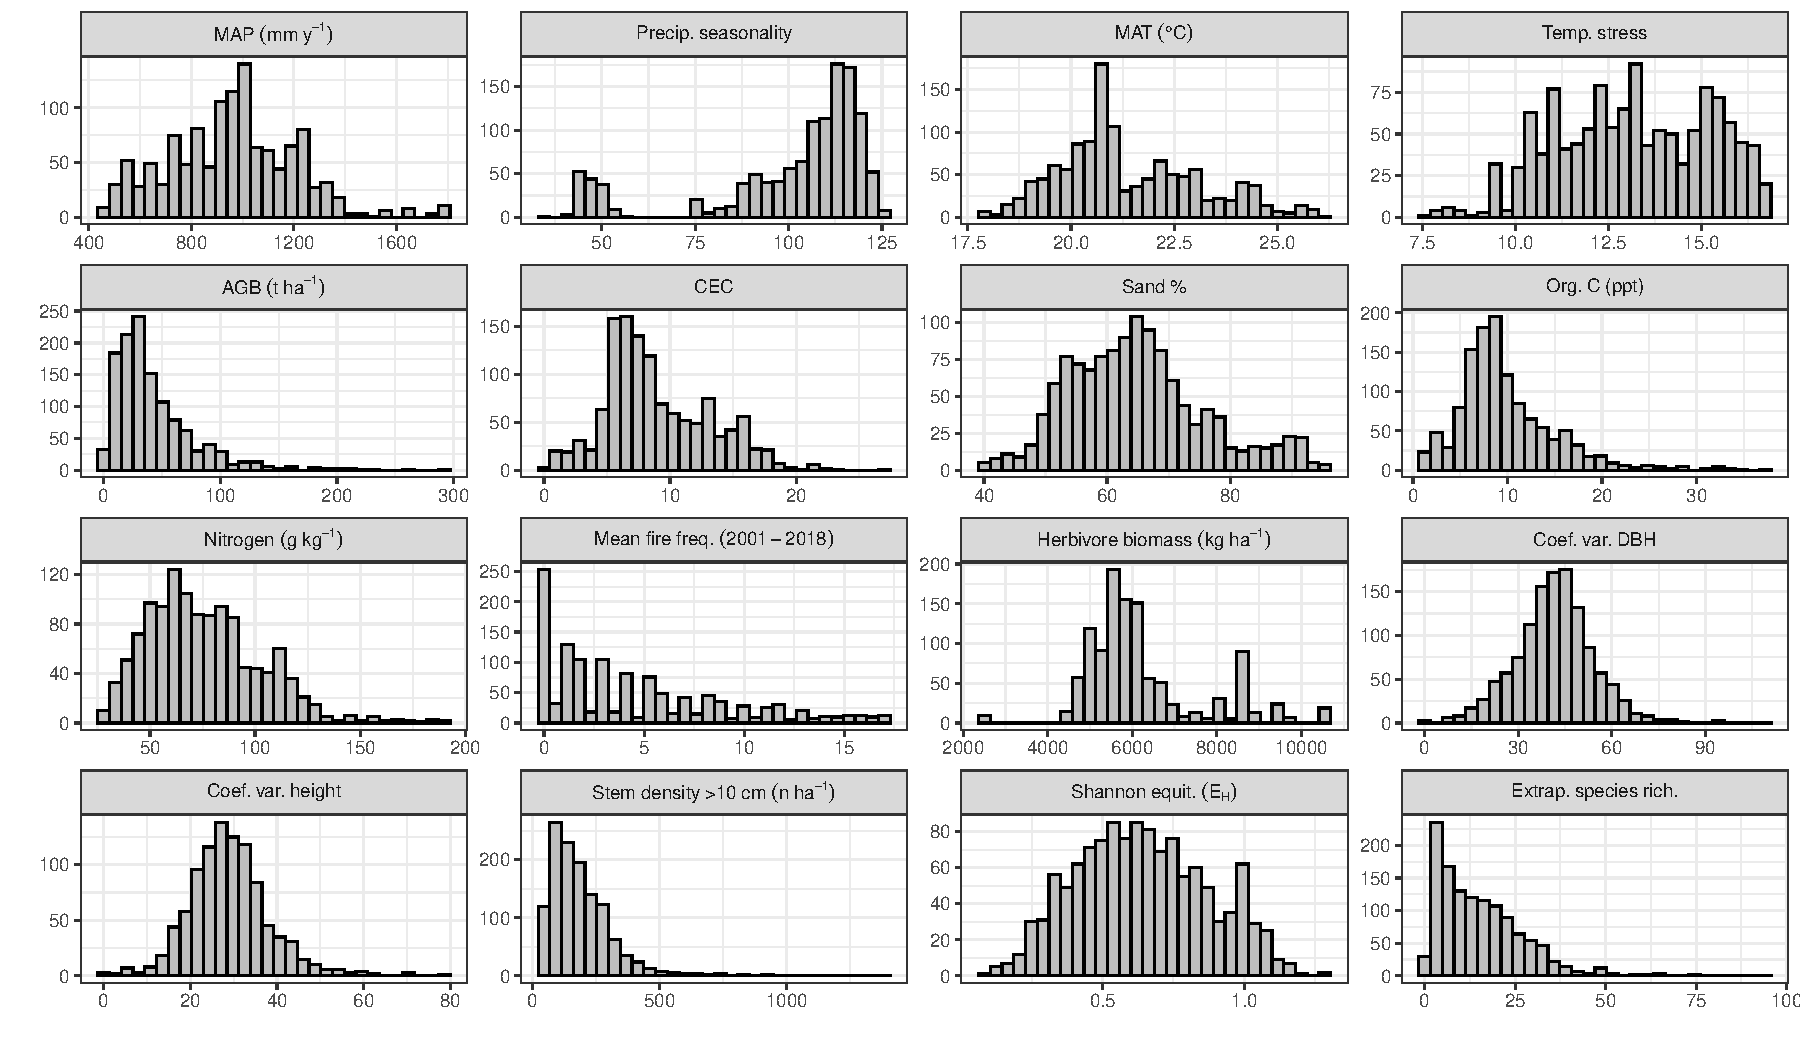
\includegraphics[width=\textwidth]{hist_raw}
	\caption{Histograms of raw untransformed observed variables used in final analyses.}
	\label{hist_raw}
\end{figure}

\begin{figure}[H]
\centering
	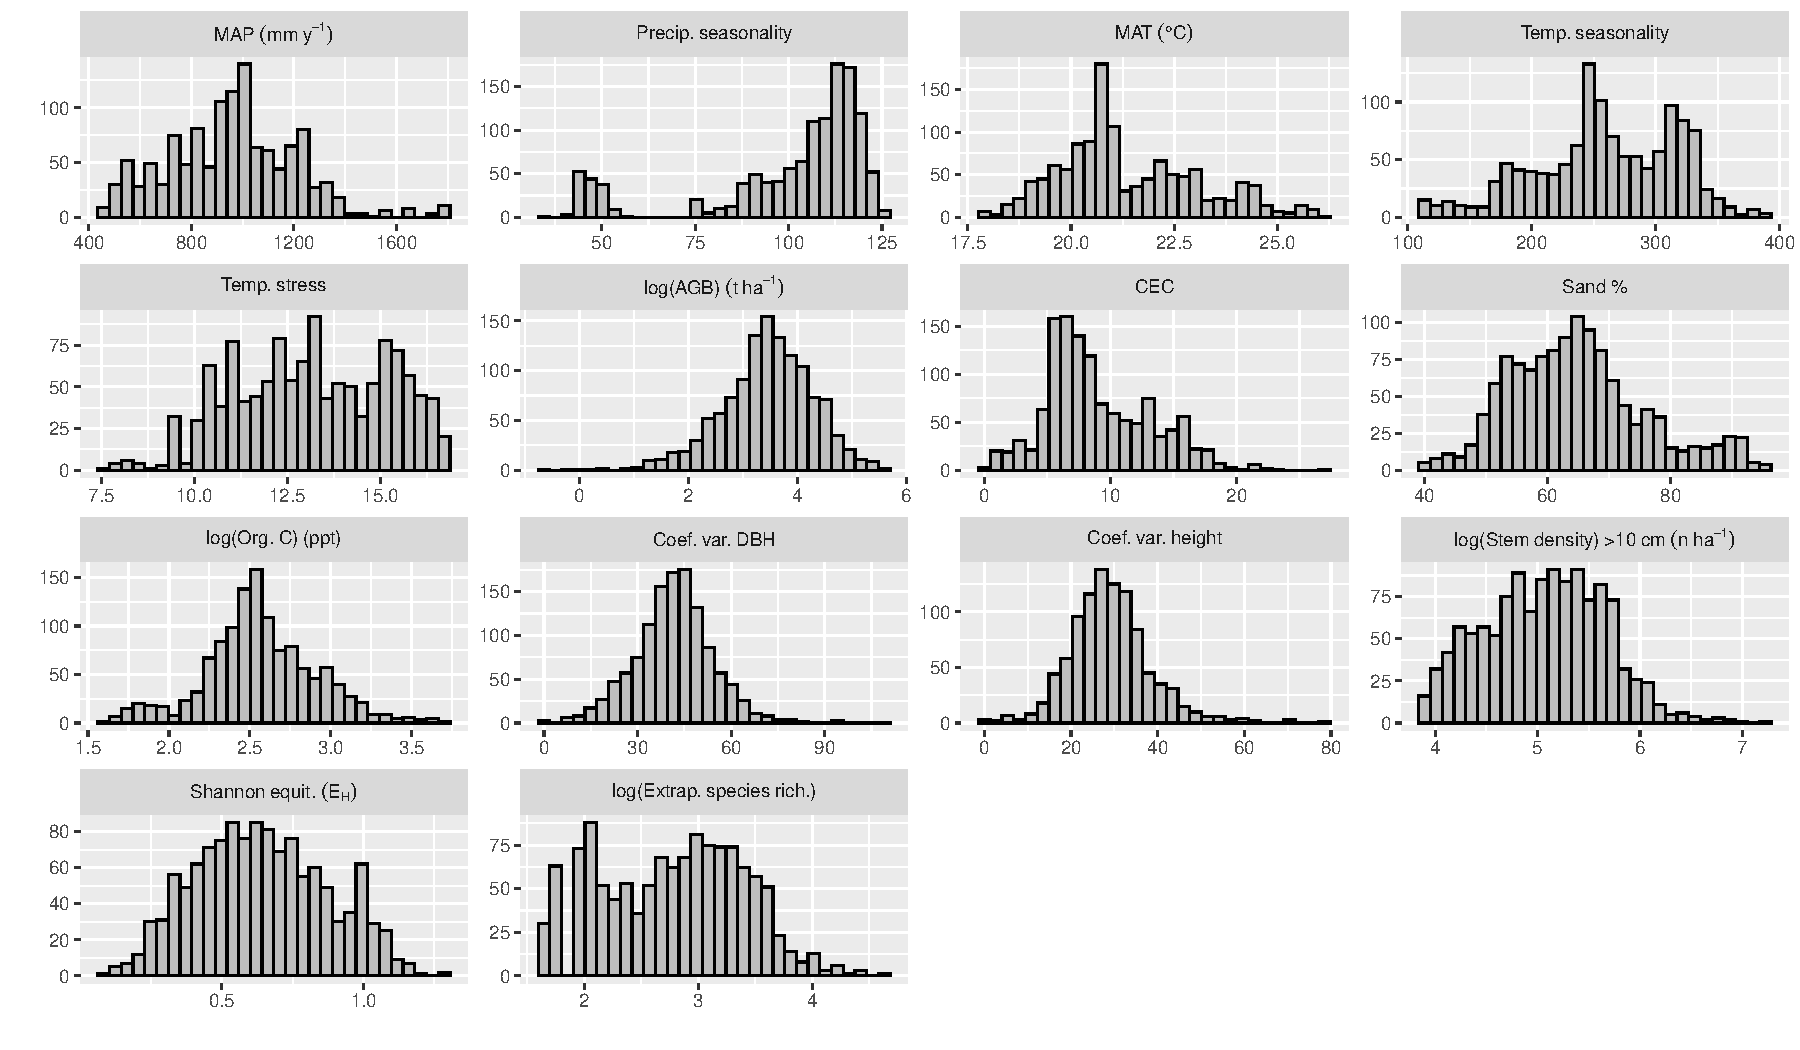
\includegraphics[width=\textwidth]{hist_trans}
	\caption{Histograms of observed variables transformed to achieve a normal frequency distribution.}
	\label{hist_trans}
\end{figure}

\appendix{}
\section{Appendix 2 - Table of correlation fit statistics} \label{appendixb}


% Table created by stargazer v.5.2.2 by Marek Hlavac, Harvard University. E-mail: hlavac at fas.harvard.edu
% Date and time: Wed, Jun 24, 2020 - 13:33:02
\begin{table}[!htbp] \centering 
  \caption{} 
  \label{corr_ci_tab} 
\begin{tabular}{@{\extracolsep{5pt}} ccccccc} 
\\[-1.8ex]\hline 
\hline \\[-1.8ex] 
x\_var & y\_var & raw.r & raw.lower & raw.upper & n & p \\ 
\hline \\[-1.8ex] 
Sand \% & Org. C (ppt) & $$-$0.620$ & $$-$0.650$ & $$-$0.580$ & $1235$ & p \textless 0.01 \\ 
Sand \% & CEC & $$-$0.510$ & $$-$0.550$ & $$-$0.470$ & $1235$ & p \textless 0.01 \\ 
Sand \% & MAP & $$-$0.500$ & $$-$0.540$ & $$-$0.460$ & $1235$ & p \textless 0.01 \\ 
Sand \% & PS & $0.350$ & $0.300$ & $0.400$ & $1235$ & p \textless 0.01 \\ 
Sand \% & MAT & $0.340$ & $0.280$ & $0.380$ & $1235$ & p \textless 0.01 \\ 
Sand \% & TS & $0.380$ & $0.330$ & $0.430$ & $1235$ & p \textless 0.01 \\ 
Sand \% & Sp. rich. & $$-$0.330$ & $$-$0.370$ & $$-$0.280$ & $1235$ & p \textless 0.01 \\ 
Sand \% & Shannon equit. & $0.250$ & $0.190$ & $0.300$ & $1235$ & p \textless 0.01 \\ 
Sand \% & Tree height CV & $$-$0.250$ & $$-$0.300$ & $$-$0.190$ & $981$ & p \textless 0.01 \\ 
Sand \% & DBH CV & $$-$0.170$ & $$-$0.230$ & $$-$0.120$ & $1233$ & p \textless 0.01 \\ 
Sand \% & Stems ha & $$-$0.100$ & $$-$0.160$ & $$-$0.050$ & $1235$ & p \textless 0.01 \\ 
Sand \% & AGB & $$-$0.270$ & $$-$0.320$ & $$-$0.220$ & $1235$ & p \textless 0.01 \\ 
Org. C (ppt) & CEC & $0.460$ & $0.410$ & $0.500$ & $1235$ & p \textless 0.01 \\ 
Org. C (ppt) & MAP & $0.440$ & $0.390$ & $0.480$ & $1235$ & p \textless 0.01 \\ 
Org. C (ppt) & PS & $$-$0.410$ & $$-$0.450$ & $$-$0.360$ & $1235$ & p \textless 0.01 \\ 
Org. C (ppt) & MAT & $$-$0.280$ & $$-$0.330$ & $$-$0.230$ & $1235$ & p \textless 0.01 \\ 
Org. C (ppt) & TS & $$-$0.280$ & $$-$0.330$ & $$-$0.230$ & $1235$ & p \textless 0.01 \\ 
Org. C (ppt) & Sp. rich. & $0.150$ & $0.090$ & $0.200$ & $1235$ & p \textless 0.01 \\ 
Org. C (ppt) & Shannon equit. & $$-$0.160$ & $$-$0.220$ & $$-$0.110$ & $1235$ & p \textless 0.01 \\ 
Org. C (ppt) & Tree height CV & $0.180$ & $0.120$ & $0.240$ & $981$ & p \textless 0.01 \\ 
Org. C (ppt) & DBH CV & $0.140$ & $0.080$ & $0.190$ & $1233$ & p \textless 0.01 \\ 
Org. C (ppt) & Stems ha & $0.090$ & $0.030$ & $0.140$ & $1235$ & p \textless 0.01 \\ 
Org. C (ppt) & AGB & $0.270$ & $0.220$ & $0.320$ & $1235$ & p \textless 0.01 \\ 
CEC & MAP & $$-$0.070$ & $$-$0.130$ & $$-$0.020$ & $1235$ & p \textless 0.01 \\ 
CEC & PS & $$-$0.590$ & $$-$0.630$ & $$-$0.550$ & $1235$ & p \textless 0.01 \\ 
CEC & MAT & $0.170$ & $0.120$ & $0.220$ & $1235$ & p \textless 0.01 \\ 
CEC & TS & $0.070$ & $0.010$ & $0.120$ & $1235$ & p \textless 0.05 \\ 
CEC & Sp. rich. & $$-$0.100$ & $$-$0.160$ & $$-$0.050$ & $1235$ & p \textless 0.01 \\ 
CEC & Shannon equit. & $$-$0.120$ & $$-$0.180$ & $$-$0.070$ & $1235$ & p \textless 0.01 \\ 
CEC & Tree height CV & $0.090$ & $0.020$ & $0.150$ & $981$ & p \textless 0.01 \\ 
CEC & DBH CV & $0.130$ & $0.080$ & $0.190$ & $1233$ & p \textless 0.01 \\ 
CEC & Stems ha & $$-$0.090$ & $$-$0.140$ & $$-$0.030$ & $1235$ & p \textless 0.01 \\ 
CEC & AGB & $0.080$ & $0.030$ & $0.140$ & $1235$ & p \textless 0.01 \\ 
MAP & PS & $$-$0.070$ & $$-$0.130$ & $$-$0.020$ & $1235$ & p \textless 0.05 \\ 
MAP & MAT & $$-$0.200$ & $$-$0.260$ & $$-$0.150$ & $1235$ & p \textless 0.01 \\ 
MAP & TS & $$-$0.770$ & $$-$0.790$ & $$-$0.740$ & $1235$ & p \textless 0.01 \\ 
MAP & Sp. rich. & $0.400$ & $0.350$ & $0.450$ & $1235$ & p \textless 0.01 \\ 
MAP & Shannon equit. & $$-$0.130$ & $$-$0.180$ & $$-$0.070$ & $1235$ & p \textless 0.01 \\ 
MAP & Tree height CV & $0.250$ & $0.190$ & $0.310$ & $981$ & p \textless 0.01 \\ 
MAP & DBH CV & $0.120$ & $0.060$ & $0.170$ & $1233$ & p \textless 0.01 \\ 
MAP & Stems ha & $0.070$ & $0.010$ & $0.120$ & $1235$ & p \textless 0.05 \\ 
MAP & AGB & $0.230$ & $0.180$ & $0.280$ & $1235$ & p \textless 0.01 \\ 
precip\_seas\_std & MAT & $0$ & $$-$0.050$ & $0.060$ & $1235$ & p = 0.95 \\ 
precip\_seas\_std & TS & $0.140$ & $0.080$ & $0.190$ & $1235$ & p \textless 0.01 \\ 
precip\_seas\_std & Sp. rich. & $0.130$ & $0.070$ & $0.180$ & $1235$ & p \textless 0.01 \\ 
precip\_seas\_std & Shannon equit. & $0.070$ & $0.010$ & $0.130$ & $1235$ & p \textless 0.05 \\ 
precip\_seas\_std & Tree height CV & $$-$0.060$ & $$-$0.120$ & $0.010$ & $981$ & p = 0.07 \\ 
precip\_seas\_std & DBH CV & $$-$0.100$ & $$-$0.150$ & $$-$0.040$ & $1233$ & p \textless 0.01 \\ 
precip\_seas\_std & Stems ha & $$-$0.030$ & $$-$0.080$ & $0.030$ & $1235$ & p = 0.33 \\ 
precip\_seas\_std & AGB & $$-$0.190$ & $$-$0.240$ & $$-$0.130$ & $1235$ & p \textless 0.01 \\ 
MAT & TS & $0.060$ & $0$ & $0.120$ & $1235$ & p \textless 0.05 \\ 
MAT & Sp. rich. & $$-$0.170$ & $$-$0.220$ & $$-$0.120$ & $1235$ & p \textless 0.01 \\ 
MAT & Shannon equit. & $0$ & $$-$0.060$ & $0.060$ & $1235$ & p = 0.98 \\ 
MAT & Tree height CV & $$-$0.040$ & $$-$0.100$ & $0.020$ & $981$ & p = 0.2 \\ 
MAT & DBH CV & $0.060$ & $0.010$ & $0.120$ & $1233$ & p \textless 0.05 \\ 
MAT & Stems ha & $$-$0.150$ & $$-$0.210$ & $$-$0.100$ & $1235$ & p \textless 0.01 \\ 
MAT & AGB & $$-$0.090$ & $$-$0.150$ & $$-$0.040$ & $1235$ & p \textless 0.01 \\ 
TS & Sp. rich. & $$-$0.440$ & $$-$0.480$ & $$-$0.390$ & $1235$ & p \textless 0.01 \\ 
TS & Shannon equit. & $0.200$ & $0.150$ & $0.250$ & $1235$ & p \textless 0.01 \\ 
TS & Tree height CV & $$-$0.210$ & $$-$0.270$ & $$-$0.150$ & $981$ & p \textless 0.01 \\ 
TS & DBH CV & $$-$0.090$ & $$-$0.150$ & $$-$0.040$ & $1233$ & p \textless 0.01 \\ 
TS & Stems ha & $$-$0.050$ & $$-$0.110$ & $0.010$ & $1235$ & p = 0.08 \\ 
TS & AGB & $$-$0.180$ & $$-$0.230$ & $$-$0.120$ & $1235$ & p \textless 0.01 \\ 
Sp. rich. & Shannon equit. & $$-$0.580$ & $$-$0.620$ & $$-$0.540$ & $1235$ & p \textless 0.01 \\ 
Sp. rich. & Tree height CV & $0.300$ & $0.250$ & $0.360$ & $981$ & p \textless 0.01 \\ 
Sp. rich. & DBH CV & $0.300$ & $0.250$ & $0.350$ & $1233$ & p \textless 0.01 \\ 
Sp. rich. & Stems ha & $0.240$ & $0.190$ & $0.300$ & $1235$ & p \textless 0.01 \\ 
Sp. rich. & AGB & $0.310$ & $0.260$ & $0.360$ & $1235$ & p \textless 0.01 \\ 
Shannon equit. & Tree height CV & $$-$0.120$ & $$-$0.190$ & $$-$0.060$ & $981$ & p \textless 0.01 \\ 
Shannon equit. & DBH CV & $$-$0.200$ & $$-$0.250$ & $$-$0.140$ & $1233$ & p \textless 0.01 \\ 
Shannon equit. & Stems ha & $$-$0.410$ & $$-$0.460$ & $$-$0.360$ & $1235$ & p \textless 0.01 \\ 
Shannon equit. & AGB & $$-$0.350$ & $$-$0.400$ & $$-$0.300$ & $1235$ & p \textless 0.01 \\ 
Tree height CV & DBH CV & $0.470$ & $0.420$ & $0.520$ & $981$ & p \textless 0.01 \\ 
Tree height CV & Stems ha & $0.010$ & $$-$0.060$ & $0.070$ & $981$ & p = 0.86 \\ 
Tree height CV & AGB & $0.240$ & $0.180$ & $0.290$ & $981$ & p \textless 0.01 \\ 
DBH CV & Stems ha & $0.110$ & $0.060$ & $0.170$ & $1233$ & p \textless 0.01 \\ 
DBH CV & AGB & $0.430$ & $0.390$ & $0.480$ & $1233$ & p \textless 0.01 \\ 
Stems ha & AGB & $0.590$ & $0.550$ & $0.620$ & $1235$ & p \textless 0.01 \\ 
\hline \\[-1.8ex] 
\end{tabular} 
\end{table} 


\section{Appendix 3 - Bivariate relationships of model variables} \label{appendixc}

\begin{figure}[H]
\centering
	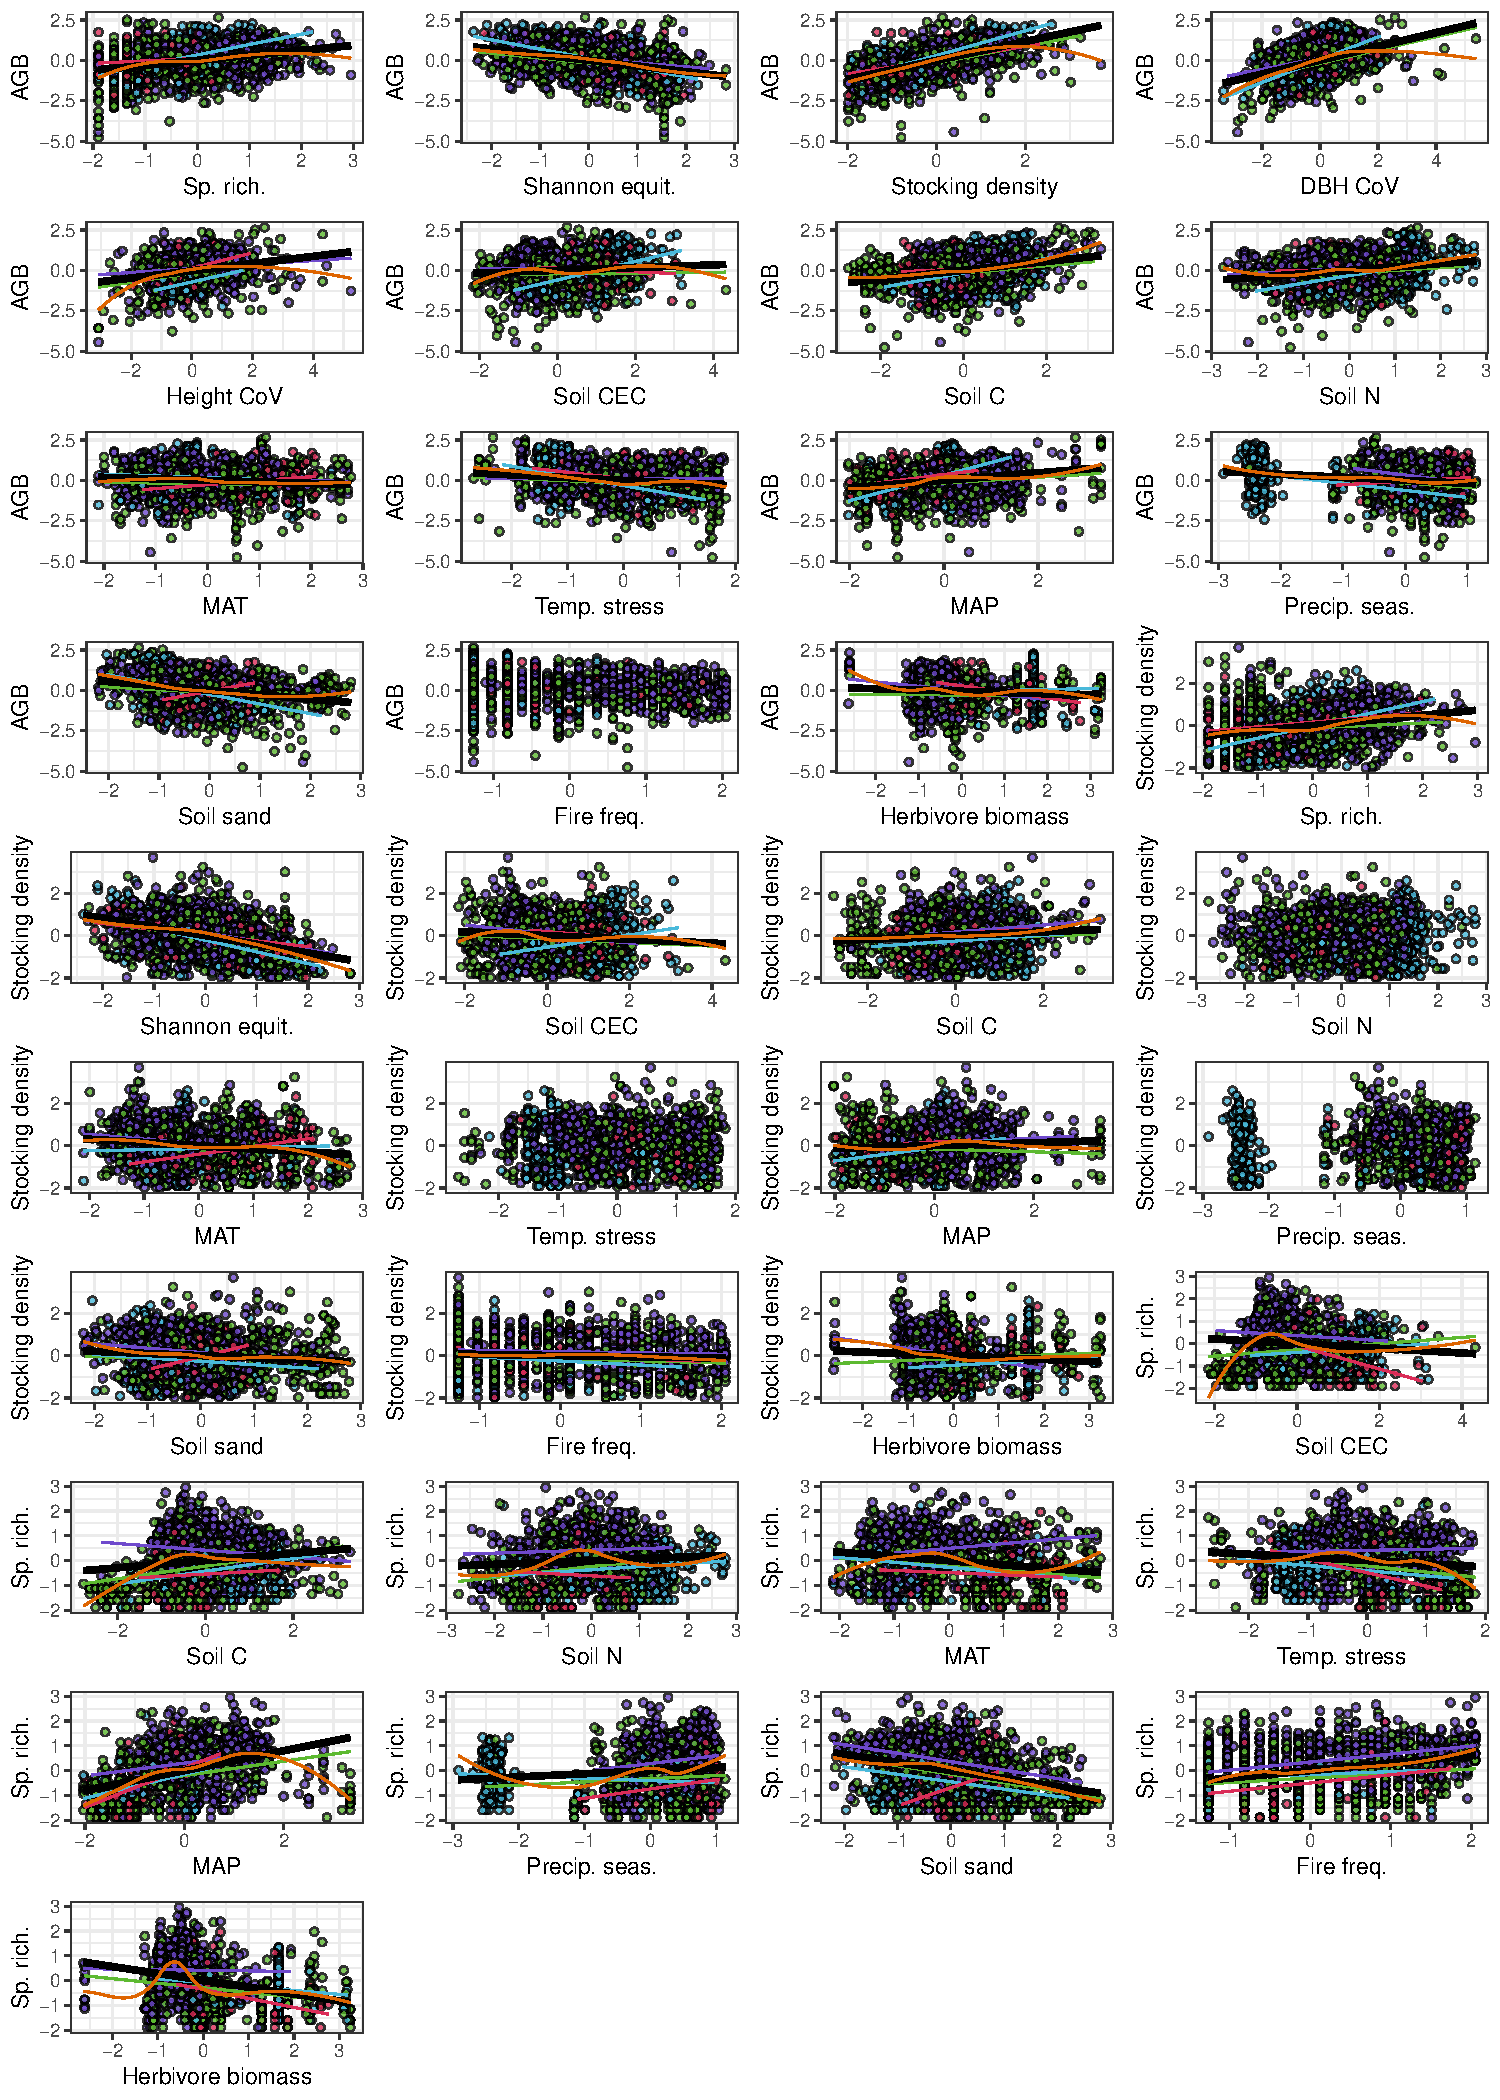
\includegraphics[width=0.9\textwidth]{bivar_lm}
	\caption{Bivariate scatter plots for each observed variable used in the SEMs, based on hypothesised paths of causality. Points are coloured according to vegetation type. A single linear regression is presented as a black line, which combines all vegetation types, separate loess trend lines are fitted for each vegetation type. An orange loess trend line is fitted for all the data. All data is standardised and variables are transformed where it was appropriate for analysis.}
	\label{bivar_lm}
\end{figure}

\section{Appendix 4 - Path coefficients for model incorporating environmental covariates} \label{appendixd}

\begin{figure}[H]
\centering
	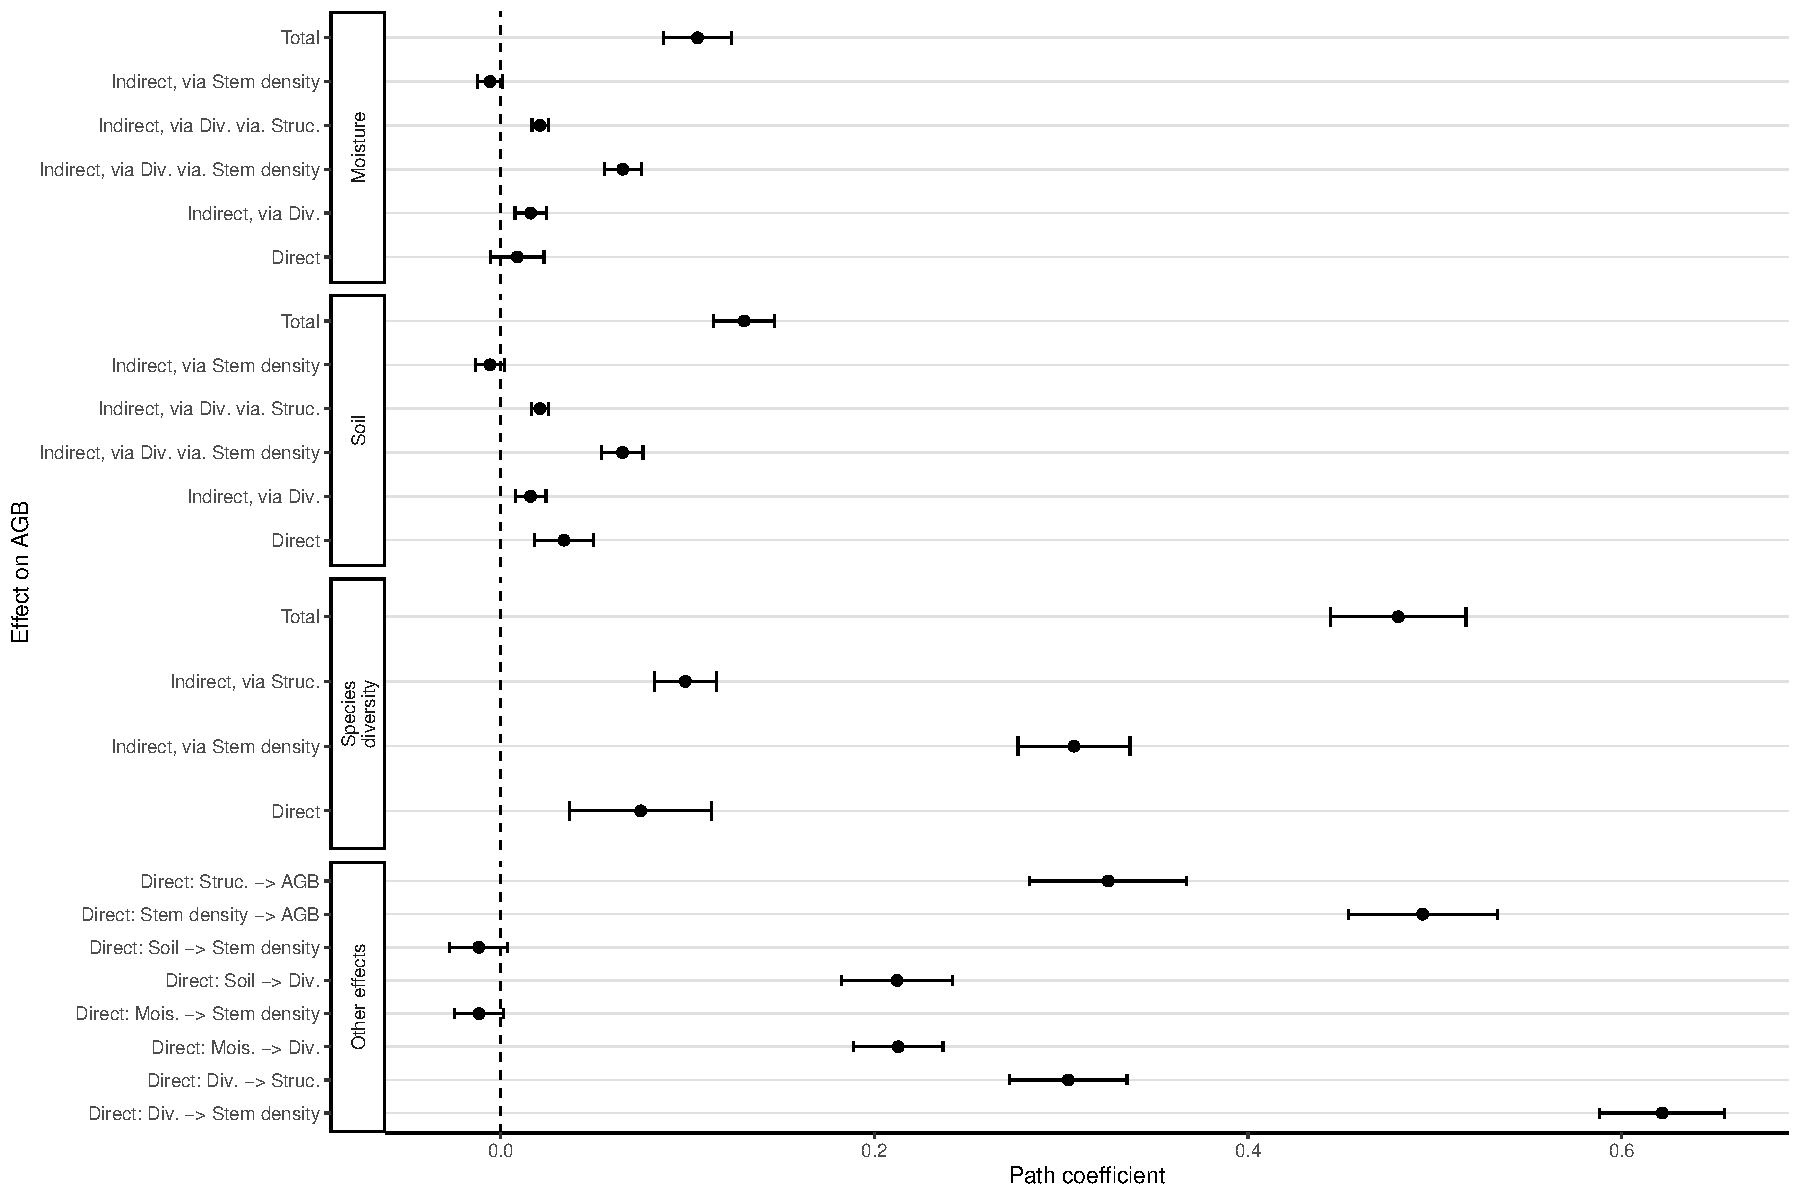
\includegraphics[width=\textwidth]{full_model_slopes}
	\caption{Unstandardised path coefficients for the full model including tree species diversity, environmental covariates and stem density. Path coefficients are $\pm1$ standard error. Path coefficients where the interval (standard error) does not overlap zero are considered to be significant effects.}
	\label{full_model_slopes}
\end{figure}

